\section{Github}
Link for the every exercises in Lab 1: \href{https://github.com/Lmonk555/lab02_micro_process_control.git}{Link}


\section{Exercise and Report}





\subsection{Exercise 1}
The first exercise show how to interface for multiple seven segment LEDs to STM32F103C6 micro-controller (MCU). Seven segment displays are common anode type, meaning that the anode of all LEDs are tied together as a single terminal and cathodes are left alone as individual pins. \\

In order to save the resource of the MCU, individual cathode pins from all the seven segment LEDs are connected together, and connect to 7 pins of the MCU. These pins are popular known as the \textbf{signal pins}. Meanwhile, the anode pin of each seven segment LEDs are controlled under a power enabling circuit, for instance, an PNP transistor. At a given time, only one seven segment LED is turned on. However, if the delay is small enough, it seems that all LEDs are enabling. \\

Implement the circuit simulation in Proteus with two 7-SEGMENT LEDs as following:

\begin{figure}[!htp]
    \centering
    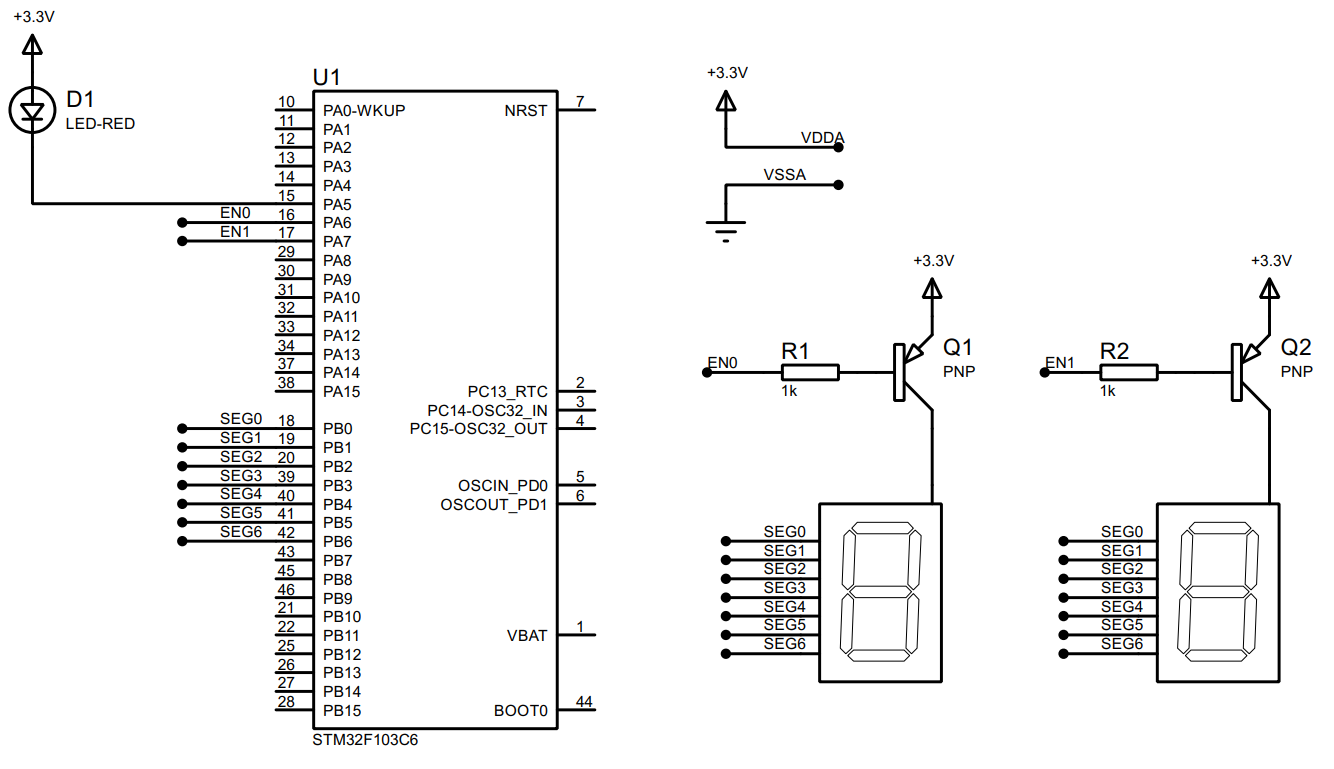
\includegraphics[width=5.5in]{pictures/bai_2/lab2_ex1a.PNG}
    \caption{\textit{Simulation schematic in Proteus}}
    \label{bai2_pic1a}
\end{figure}
Components used in the schematic are listed bellow:
\begin{itemize}
    \item 7SEG-COM-ANODE (connected from PB0 to PB6)
    \item LED-RED
    \item PNP
    \item RES
    \item STM32F103C6
\end{itemize}


Students are proposed to use the function \textbf{display7SEG(int num)} in the Lab 1 in this exercise. Implement the source code in the interrupt callback function to display number \textbf{"1"} on the first seven segment and number \textbf{"2"} for second one. The switching time between 2 LEDs is half of second. \\

\textbf{Report 1: } Capture your schematic from Proteus and show in the report.\\

\begin{figure}[H]
    \centering
    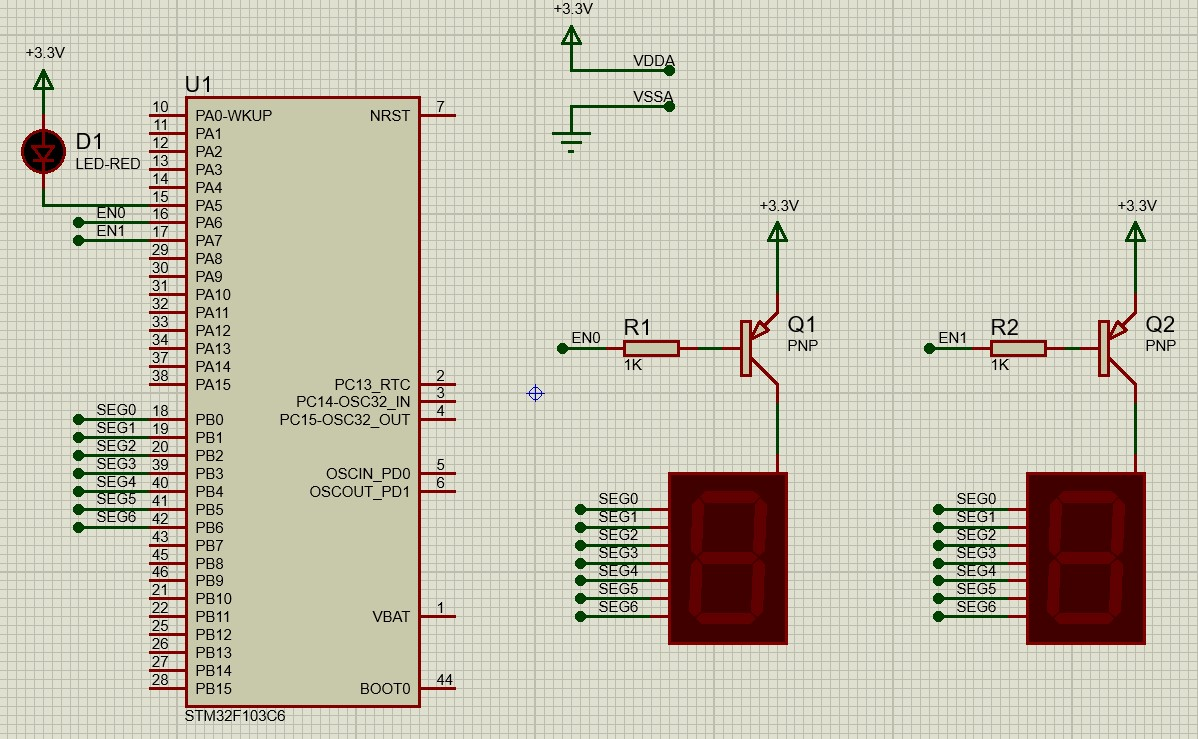
\includegraphics[width=0.8\linewidth]{pictures/schematic_ex01.jpg}
    \caption{{\textit{Proteus schematic for two 7-segment LEDs}}}
    \label{schematic_ex01}
\end{figure}

\textbf{Report 2: } Present your source code in the \textbf{HAL\_TIM\_PeriodElapsedCallback} function.\\

- Before implementing function \texttt{void HAL\_TIM\_PeriodElapsedCallback(TIM\_HandleTypeDef *htim){}}, we need to initialize essential variables and functions from Lab 1.

\textbf{\textit{Note:}} This should be written in \texttt{/* USER CODE BEGIN 0 */} block as we define them globally and easier to look out afterward.

\begin{lstlisting}[language=c,caption={Initial implementation for Exercise 01}]
/* USER CODE BEGIN 0 */
typedef struct
{
    GPIO_TypeDef *port;
    uint16_t pin;
} SegPin;


SegPin segments[] =
{
    { SEG0_GPIO_Port, SEG0_Pin },
    { SEG1_GPIO_Port, SEG1_Pin },
    { SEG2_GPIO_Port, SEG2_Pin },
    { SEG3_GPIO_Port, SEG3_Pin },
    { SEG4_GPIO_Port, SEG4_Pin },
    { SEG5_GPIO_Port, SEG5_Pin },
    { SEG6_GPIO_Port, SEG6_Pin },
};


GPIO_PinState digitPatterns[10][7] =
{
    { RESET, RESET, RESET, RESET, RESET, RESET, SET   },	// 0
    { SET,   RESET, RESET, SET,   SET,   SET,   SET   },	// 1
    { RESET, RESET, SET,   RESET, RESET, SET,   RESET },	// 2
    { RESET, RESET, RESET, RESET, SET,   SET,   RESET },	// 3
    { SET,   RESET, RESET, SET,   SET,   RESET, RESET },	// 4
    { RESET, SET,   RESET, RESET, SET,   RESET, RESET },	// 5
    { RESET, SET,   RESET, RESET, RESET, RESET, RESET },	// 6
    { RESET, RESET, RESET, SET,   SET,   SET,   SET   },	// 7
    { RESET, RESET, RESET, RESET, RESET, RESET, RESET },	// 8
    { RESET, RESET, RESET, RESET, SET,   RESET, RESET },	// 9
};


void display7SEG(int num)
{
    if (num < 0 || num > 9) return;

    HAL_GPIO_WritePin(EN0_GPIO_Port, EN0_Pin, GPIO_PIN_SET);
    HAL_GPIO_WritePin(EN1_GPIO_Port, EN1_Pin, GPIO_PIN_SET);

    for (int i = 0; i < 7; i++)
        HAL_GPIO_WritePin(segments[i].port, segments[i].pin, digitPatterns[num][i]);
}

int counter = 50;
int state = 0;

/* USER CODE END 0 */
\end{lstlisting}

\newpage
- Now we can go for implementation:

\begin{lstlisting}[language=c,caption={Exercise 01 source code in HAL\_TIM\_PeriodElapsedCallback function}]
void HAL_TIM_PeriodElapsedCallback(TIM_HandleTypeDef *htim)
{
    counter--;
    if(counter <= 0)
    {
        counter = 50;
        HAL_GPIO_TogglePin(LED_GPIO_Port, LED_Pin);


        if (state == 0)
        {
            display7SEG(1);
            HAL_GPIO_WritePin(EN0_GPIO_Port, EN0_Pin, GPIO_PIN_RESET);
            state = 1;
        }
        else
        {
            dis play7SEG(2);
            HAL_GPIO_WritePin(EN1_GPIO_Port, EN1_Pin, GPIO_PIN_RESET);
            state = 0;
        }
    }
}
\end{lstlisting}

\textbf{Short question: } What is the frequency of the scanning process?

- Each seven-segment LED stays on for $T_s = 0.5\,\text{s}$. With 2 LEDs, one full scan cycle (LED 1, then LED 2) takes $2 \times T_s = 1\,\text{s}$.

\[
f = \frac{1}{2 \cdot T_s} = \frac{1}{2 \cdot 0.5} = 1\,\text{Hz}
\]

- This matches the lab's formula $f = \frac{1}{N \cdot T_s}$, where $N$ is the number of LEDs.

\textbf{Therefore, the scanning frequency is 1 Hz.}










\subsection{Exercise 2}
Extend to 4 seven segment LEDs and two LEDs (connected to PA4, labeled as \textbf{DOT}) in the middle as following:

\begin{figure}[H]
    \centering
    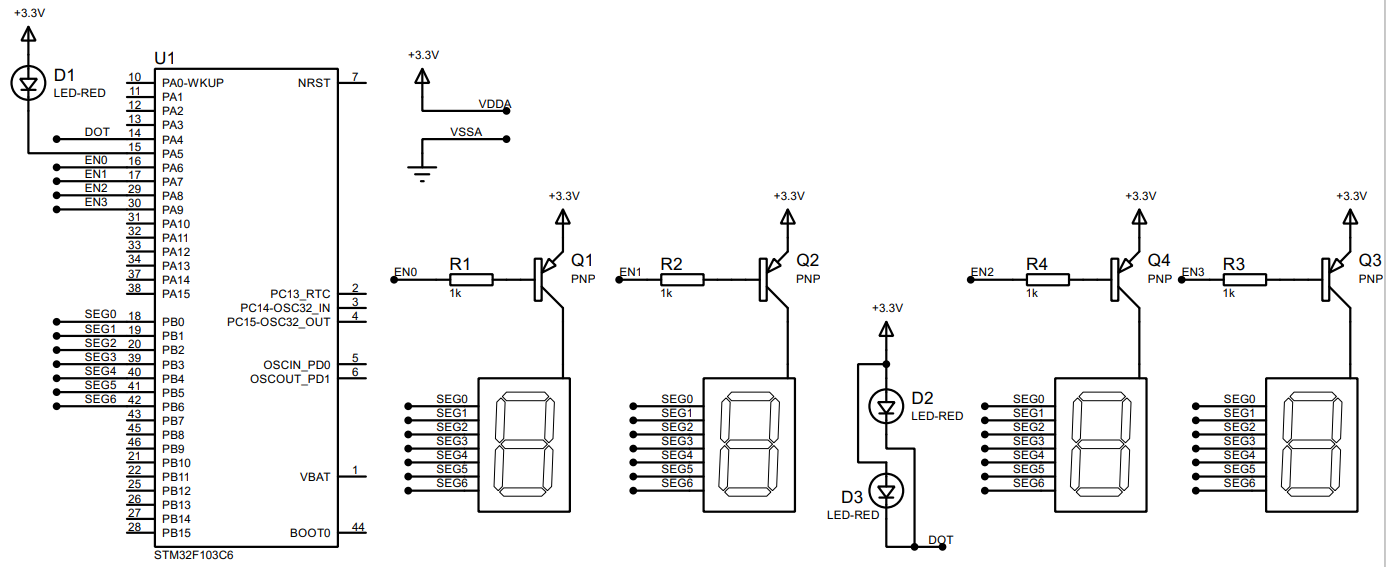
\includegraphics[width=5.5in]{pictures/bai_2/lab2_ex2a.PNG}
    \caption{\textit{Simulation schematic in Proteus}}
    \label{bai2_pic2a}
\end{figure}

Blink the two LEDs every second. Meanwhile, number 3 is displayed on the third seven segment and number 0 is displayed on the last one (to present 12 hour and a half). The switching time for each seven segment LED is also a half of second (500ms). \textbf{Implement your code in the timer interrupt function.}\\

\textbf{Report 1: } Capture your schematic from Proteus and show in the report.\\
\textbf{\textit{Note: }} \textit{As the exercise 09 and 10 add more components but it does not affect the schematic that we use for Exercise 3.2 to 3.7, we will submit the final schematic that can use all \texttt{.hex} files from 3.2 to 3.10}

\begin{figure}[H]
    \centering
    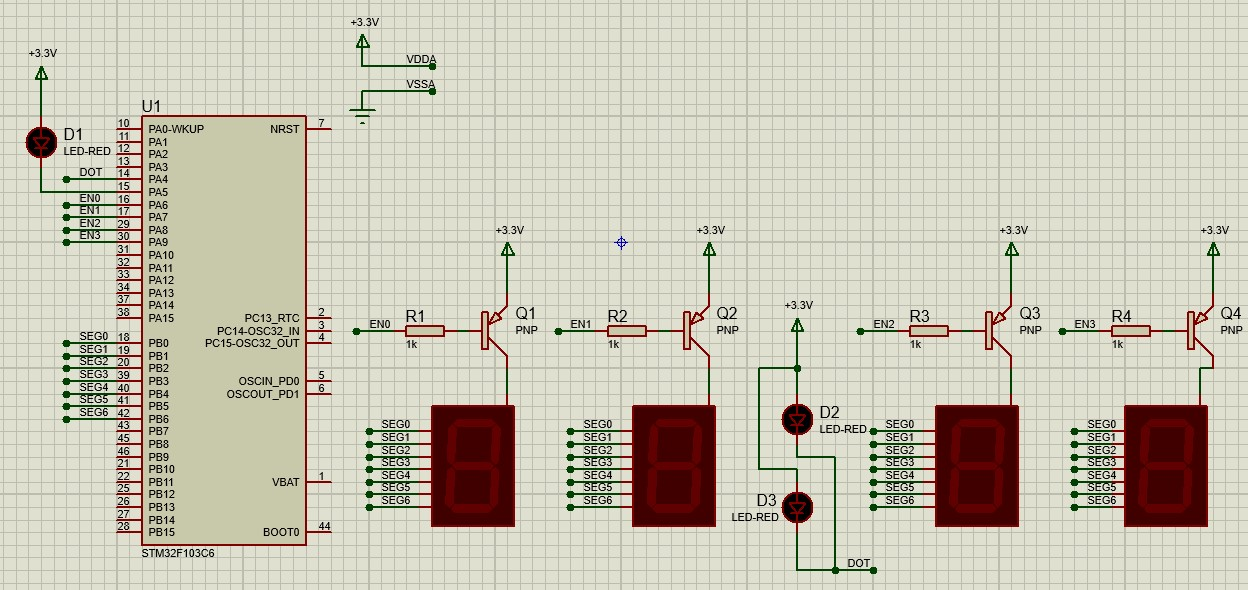
\includegraphics[width=0.8\linewidth]{pictures/schematic_ex02_08.jpg}
    \caption{{\textit{Proteus schematic for four 7-segment LEDs}}}
    \label{schematic_ex02}
\end{figure}

\textbf{Report 2: } Present your source code in the \textbf{HAL\_TIM\_PeriodElapsedCallback} function.\\

- As the increasing of 7-segment LEDs, we will re-define some variables and update \texttt{void display7SEG(int num)}:

\begin{lstlisting}[language=c,caption={Initial implementation for Exercise 02}]
/* USER CODE BEGIN 0 */

// RE-USE Exercise 01 structures

void display7SEG(int num)
{
    if (num < 0 || num > 9) return;

    HAL_GPIO_WritePin(EN0_GPIO_Port, EN0_Pin, GPIO_PIN_SET);
    HAL_GPIO_WritePin(EN1_GPIO_Port, EN1_Pin, GPIO_PIN_SET);
    HAL_GPIO_WritePin(EN2_GPIO_Port, EN2_Pin, GPIO_PIN_SET);
    HAL_GPIO_WritePin(EN3_GPIO_Port, EN3_Pin, GPIO_PIN_SET);

    for (int i = 0; i < 7; i++)
        HAL_GPIO_WritePin(segments[i].port, segments[i].pin, digitPatterns[num][i]);
}


// From exercise 3.2
int digit_counter = 50;
int dot_counter   = 100;
int state = 0;
int digits[4] = {1, 2, 3, 0};

/* USER CODE END 0 */
\end{lstlisting}

\newpage
\begin{lstlisting}[language=c,caption={Exercise 02 source code in HAL\_TIM\_PeriodElapsedCallback function}]
void HAL_TIM_PeriodElapsedCallback(TIM_HandleTypeDef *htim)
{
    counter--;
    if(counter <= 0)
    {
        counter = 50;
        HAL_GPIO_TogglePin(LED_GPIO_Port, LED_Pin);


        if (state == 0)
        {
            display7SEG(1);
            HAL_GPIO_WritePin(EN0_GPIO_Port, EN0_Pin, GPIO_PIN_RESET);
            state = 1;
        }
        else
        {
            display7SEG(2);
            HAL_GPIO_WritePin(EN1_GPIO_Port, EN1_Pin, GPIO_PIN_RESET);
            state = 0;
        }
    }
}
\end{lstlisting}

\textbf{Short question: } What is the frequency of the scanning process?\\

- Applying the solve from Exercise 3.1, for Exercise 3.2 with 4 LEDs and $T_s = 0.5\,\text{s}$, it would be $\frac{1}{4 \cdot 0.5} = 0.5\,\text{Hz}$.










\newpage
\subsection{Exercise 3}
Implement a function named \textbf{update7SEG(int index)}. An array of 4 integer numbers are declared in this case. The code skeleton in this exercise is presented as following:

\begin{lstlisting}[caption=An example for your source code]
const int MAX_LED = 4;
int index_led = 0;
int led_buffer[4] = {1, 2, 3, 4};
void update7SEG(int index){
    switch (index){
        case 0:
            //Display the first 7SEG with led_buffer[0]
            break;
        case 1:
            //Display the second 7SEG with led_buffer[1]
            break;
        case 2:
            //Display the third 7SEG with led_buffer[2]
            break;
        case 3:
            //Display the forth 7SEG with led_buffer[3]
            break;
        default:
            break;
    }
}
\end{lstlisting}

This function should be invoked in the timer interrupt, e.g update7SEG(index\_led++). The variable \textbf{index\_led} is updated to stay in a valid range, which is from 0 to 3. \\

\textbf{Report 1: } Present the source code of the update7SEG function. \\

\begin{lstlisting}[language=c,caption={Source code of the update7SEG function.}]
void update7SEG(int index)
{
    switch (index)
    {
        case 0:
            display7SEG(led_buffer[0]);
            HAL_GPIO_WritePin(EN0_GPIO_Port, EN0_Pin, GPIO_PIN_RESET);
            break;
        case 1:
            display7SEG(led_buffer[1]);
            HAL_GPIO_WritePin(EN1_GPIO_Port, EN1_Pin, GPIO_PIN_RESET);
            break;
        case 2:
            display7SEG(led_buffer[2]);
            HAL_GPIO_WritePin(EN2_GPIO_Port, EN2_Pin, GPIO_PIN_RESET);
            break;
        case 3:
            display7SEG(led_buffer[3]);
            HAL_GPIO_WritePin(EN3_GPIO_Port, EN3_Pin, GPIO_PIN_RESET);
            break;
        default:
            break;
    }
}
\end{lstlisting}

\textbf{Report 2: } Present the source code in the HAL\_TIM\_PeriodElapsedCallback.\\

\begin{lstlisting}[language=c,caption={Source code in the HAL\_TIM\_PeriodElapsedCallback function.}]
void HAL_TIM_PeriodElapsedCallback(TIM_HandleTypeDef *htim)
{
    dot_counter--;
    if (dot_counter <= 0)
    {
        dot_counter = 100;
        HAL_GPIO_TogglePin(DOT_GPIO_Port, DOT_Pin);
    }

    digit_counter--;
    if (digit_counter <= 0)
    {
        digit_counter = 50;
        update7SEG(index_led++);
        HAL_GPIO_TogglePin(LED_GPIO_Port, LED_Pin);


        if (index_led >= MAX_LED)
            index_led = 0;
    }
}
\end{lstlisting}

Students are proposed to change the values in the \textbf{led\_buffer} array for unit test this function, which is used afterward.

- Changing \texttt{int led\_buffer[4] = {1, 2, 3, 4};} into => \texttt{int led\_buffer[4] = {6, 7, 6, 7};} works perfectly fine. We mention the two buffer in 2 files: \texttt{ex03\_1.hex} and \texttt{ex03\_2.hex}.










\subsection{Exercise 4}
Change the period of invoking update7SEG function in order to set the frequency of 4 seven segment LEDs to 1Hz. The DOT is still blinking every second.\\

- We already knew that the frequency of the scanning process from Exercise 3.2 is $f = 0.5\,\text{Hz}$. Using the formula $f = \frac{1}{N \cdot T_s}$ and applying $f = 1\,\text{Hz}$, we will get $T_s = 0.25\,\text{s} = 250\, \text{ms}$.

- With a $10\, \text{ms}$ timer interrupt, $\frac{250\, \text{ms}}{10\, \text{ms}} = 25$. Therefore, we have to change \texttt{digit\_counter = 25} in both \texttt{/* USER CODE BEGIN 0 */} and \texttt{void HAL\_TIM\_PeriodElapsedCallback(TIM\_HandleTypeDef *htim){}} \\

\textbf{Report 1: } Present the source code in the \textbf{HAL\_TIM\_PeriodElapsedCallback}. \\

\begin{lstlisting}[language=c,caption={Source code in the HAL\_TIM\_PeriodElapsedCallback function.}]
void HAL_TIM_PeriodElapsedCallback(TIM_HandleTypeDef *htim)
{
    dot_counter--;
    if (dot_counter <= 0)
    {
        dot_counter = 100;
        HAL_GPIO_TogglePin(DOT_GPIO_Port, DOT_Pin);
    }

    digit_counter--;
    if (digit_counter <= 0)
    {
        digit_counter = 25;
        update7SEG(index_led++);
        HAL_GPIO_TogglePin(LED_GPIO_Port, LED_Pin);


        if (index_led >= MAX_LED)
            index_led = 0;
    }
}
\end{lstlisting}










\subsection{Exercise 5}
Implement a digital clock with \textbf{hour} and \textbf {minute} information displayed by 2 seven segment LEDs. The code skeleton in the \textbf{main} function is presented as follows:
\begin{lstlisting}[caption=An example for your source code]
int hour = 15, minute = 8, second = 50;

while(1){
    second++;
    if (second >= 60){
        second = 0;
        minute++;
    }
    if(minute >= 60){
        minute = 0;
        hour++;
    }
    if(hour >=24){
        hour = 0;
    }
    updateClockBuffer();
    HAL_Delay(1000);
}
\end{lstlisting}

The function \textbf{updateClockBuffer} will generate values for the array \textbf{led\_buffer} according to the values of hour and minute. In the case these values are 1 digit number, digit 0 is added. \\

\textbf{Report 1: } Present the source code in the \textbf{updateClockBuffer} function.

\begin{lstlisting}[language=c,caption={Source code in the updateClockBuffer function.}]
void updateClockBuffer(void)
{
    led_buffer[0] = hour / 10;     // tens of hour
    led_buffer[1] = hour % 10;     // units of hour
    led_buffer[2] = minute / 10;   // tens of minute
    led_buffer[3] = minute % 10;   // units of minute
}
\end{lstlisting}








\subsection{Exercise 6}
The main target from this exercise to reduce the complexity (or reduce code processing) in the timer interrupt. The time consumed in the interrupt can lead to the nested interrupt issue, which can crash the whole system. A simple solution can disable the timer whenever the interrupt occurs, the enable it again. However, the real-time processing is not guaranteed anymore.\\

In this exercise, a software timer is created and its counter is count down every timer interrupt is raised (every 10ms). By using this timer, the \textbf{Hal\_Delay(1000)} in the main function is removed. In a MCU system, non-blocking delay is better than blocking delay. The details to create a software timer are presented bellow. The source code is added to your current program, \textbf{do not delete the source code you have on Exercise 5.}\\

\textbf{Step 1: } Declare variables and functions for a software timer, as following:
\begin{lstlisting}[caption=Software timer based timer interrupt]
/* USER CODE BEGIN 0 */
int timer0_counter = 0;
int timer0_flag = 0;
int TIMER_CYCLE = 10;
void setTimer0(int duration){
	timer0_counter = duration /TIMER_CYCLE;
	timer0_flag = 0;
}
void timer_run(){
	if(timer0_counter > 0){
		timer0_counter--;
		if(timer0_counter == 0) timer0_flag = 1;
	}
}
/* USER CODE END 0 */
\end{lstlisting}

Please change the \textbf{TIMER\_CYCLE} to your timer interrupt period. In the manual code above, it is \textbf{10ms}. \\

\textbf{Step 2: } The \textbf{timer\_run()} is invoked in the timer interrupt as following:

\begin{lstlisting}[caption=Software timer based timer interrupt]
void HAL_TIM_PeriodElapsedCallback(TIM_HandleTypeDef *htim){
	
	timer_run();
	
	//YOUR OTHER CODE
}
\end{lstlisting}

\textbf{Step 3: } Use the timer in the main function by invoked setTimer0 function, then check for its flag (timer0\_flag). An example to blink an LED connected to PA5 using software timer is shown as follows:
\begin{lstlisting}[caption=Software timer is used in main fuction to blink the LED]
setTimer0(1000);
while (1){
    if(timer0_flag == 1){
        HAL_GPIO_TogglePin(LED_RED_GPIO_Port, LED_RED_Pin);
        setTimer0(2000);
    }
}
\end{lstlisting}

\textbf{\textit{Note: }} in order to stimulate successfully, make sure to not have \texttt{HAL\_GPIO\_TogglePin(LED\_GPIO\_Port, LED\_Pin);} in \texttt{void HAL\_TIM\_PeriodElapsedCallback(TIM\_HandleTypeDef *htim)}, since we using the same code from exercise 3.5 (which is also from exercise 3.4). \\

\textbf{Report 1: } if in line 1 of the code above is miss, what happens after that and why?\\

- The LED never blinks, or likely not toggle depending on its intial state.

- Reason: \texttt{timer0\_counter} and \texttt{timer0\_flag} both start at 0, and \texttt{timer\_run()} does nothing while the counter is 0. The flag therefore never becomes 1, the if is never true, and \texttt{setTimer0(2000)} is never reached. \\

\textbf{Report 2: } if in line 1 of the code above is changed to setTimer0(1), what happens after that and why?\\

- The LED never blinks, same as Report 1.

- \texttt{timer0\_counter = duration / TIMER\_CYCLE;} = 1 / 10 = 0 because of integer division, so the counter starts at 0, \texttt{timer\_run()} never decrements it, and the flag never gets set. Any duration smaller than \texttt{TIMER\_CYCLE} (= 10 ms) rounds down to 0. \\

\textbf{Report 3: } if in line 1 of the code above is changed to setTimer0(10), what is changed compared to 2 first questions and why?\\

- The LED works.

- \texttt{timer0\_counter} = 10 / 10 = 1, so after the next interrupt (10 ms) the counter reaches 0 and \texttt{timer0\_flag} = 1. The LED toggles almost immediately, then \texttt{setTimer0(2000)} takes over, so it toggles every 2s afterwards. Compared with the first two cases, which never blink, this one blinks; compared with \texttt{setTimer0(1000)}, the only difference is that the first toggle happens after 10 ms instead of 1s. \\










\subsection{Exercise 7}
Upgrade the source code in Exercise 5 (update values for hour, minute and second) by using the software timer and remove the HAL\_Delay function at the end. Moreover, the DOT (connected to PA4) of the digital clock is also moved to main function. \\

\textbf{Report 1: } Present your source code in the while loop on main function.

\begin{lstlisting}[language=c,caption={Source code in the while loop on main function.}]
while (1)
{
	if (timer0_flag == 1)
	{
		setTimer0(1000);

		second++;
		if (second >= 60) { second = 0; minute++; }
		if (minute >= 60) { minute = 0; hour++; }
		if (hour >= 24)   { hour = 0; }

		HAL_GPIO_TogglePin(DOT_GPIO_Port, DOT_Pin);
	}
	updateClockBuffer();
}
\end{lstlisting}








\subsection{Exercise 8}
Move also the update7SEG() function from the interrupt  timer to the main. Finally, the timer interrupt only used to handle  software timers. All processing (or complex computations) is move to an infinite loop on the main function, optimizing the complexity of the interrupt  handler function.\\

\textbf{Report 1: } Present your source code in the the main function. In the case more extra functions are used (e.g. the second software timer), present them in the report as well.\\

- As we move \texttt{update7SEG()} to \texttt{int main(void)}, we have to add a second software time:

\begin{lstlisting}[language=c,caption={Updating global variables and functions}]
/* USER CODE BEGIN 0 */
//###################################################
// From exercise 3.6 (to 3.10)

int timer0_counter = 0, timer0_flag = 0;	// DOT tick
int timer1_counter = 0, timer1_flag = 0;	// digit scanning (from 3.8)
int TIMER_CYCLE = 10;


void setTimer0(int duration) { timer0_counter = duration / TIMER_CYCLE;	timer0_flag = 0; }
void setTimer1(int duration) { timer1_counter = duration / TIMER_CYCLE; timer1_flag = 0; }


void timer_run()
{
	if(timer0_counter > 0) { timer0_counter--; if(timer0_counter == 0) timer0_flag = 1;	}
    if(timer1_counter > 0) { timer1_counter--; if(timer1_counter == 0) timer1_flag = 1; }
}
/* USER CODE END 0 */

\end{lstlisting}

- Then we remove everything from \texttt{void HAL\_TIM\_PeriodElapsedCallback(TIM\_HandleTypeDef *htim)} but leave only \texttt{timer\_run();}

\begin{lstlisting}[language=c,caption={Updating void HAL\_TIM\_PeriodElapsedCallback(TIM\_HandleTypeDef *htim)}]
void HAL_TIM_PeriodElapsedCallback(TIM_HandleTypeDef *htim)
{
	// NO REMOVE FOR EXERCISE 3.6 (and later exercises)
	timer_run();
}
\end{lstlisting}

- Finally, we can implement the while loop.

\begin{lstlisting}[language=c,caption={Source code in the while loop on main function.)}]
while (1)
{
	if (timer0_flag == 1)
	{
		setTimer0(1000);

		second++;
		if (second >= 60) { second = 0; minute++; }
		if (minute >= 60) { minute = 0; hour++; }
		if (hour >= 24)   { hour = 0; }

		HAL_GPIO_TogglePin(DOT_GPIO_Port, DOT_Pin);
	}
	updateClockBuffer();


    if (timer1_flag == 1)
    {
        setTimer1(250);

        update7SEG(index_led++);
        HAL_GPIO_TogglePin(LED_GPIO_Port, LED_Pin);
        if (index_led >= MAX_LED) index_led = 0;
    }
}
\end{lstlisting}










\subsection{Exercise 9}

This is an extra works for this lab. A LED Matrix is added to the system. A reference design is shown in figure bellow:
\begin{figure}[!htp]
    \centering
    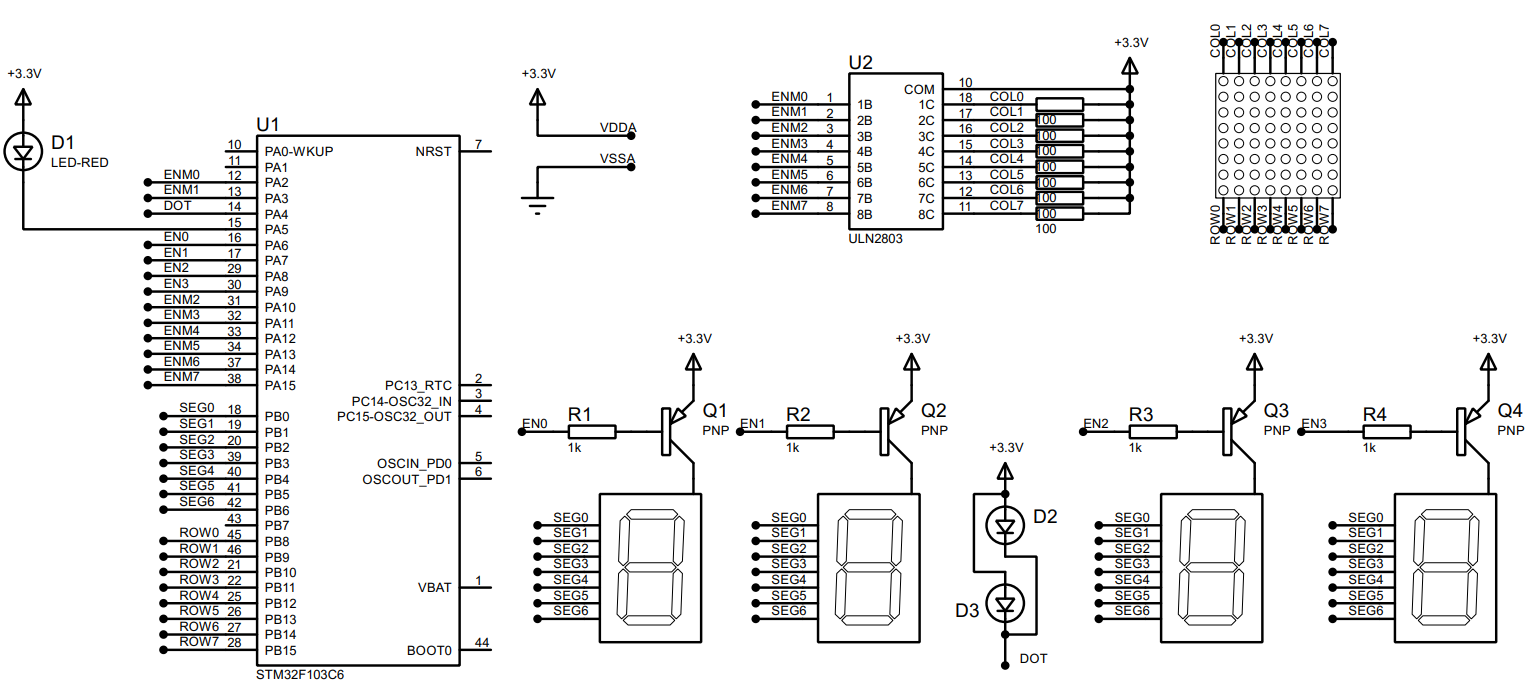
\includegraphics[width=5.5in]{pictures/bai_2/lab2_m4.PNG}
    \caption{\textit{LED matrix is added to the simulation}}
    \label{bai2_pic9}
\end{figure}

In this schematic, two new components are added, including the \textbf{MATRIX-8X8-RED} and \textbf{ULN2803}, which is an NPN transistor array to enable the power supply for a column of the LED matrix. Students can change the enable signal (from ENM0 to  ENM7) if needed. Finally, the data signal (from ROW0 to ROW7) is connected to PB8 to PB15. \\

\textbf{Report 1: } Present the schematic of your system by capturing the screen in Proteus.\\

\textbf{\textit{Note: }} When we were building the schematic on Proteus, we found out that the "just-take-out" \texttt{MATRIX-8X8-RED} was upside down to the one in \textit{Figure 2.5}. Therefore, we decided to change the wires to match with the default \texttt{MATRIX-8X8-RED} in Proteus.\\

\begin{figure}[H]
    \centering
    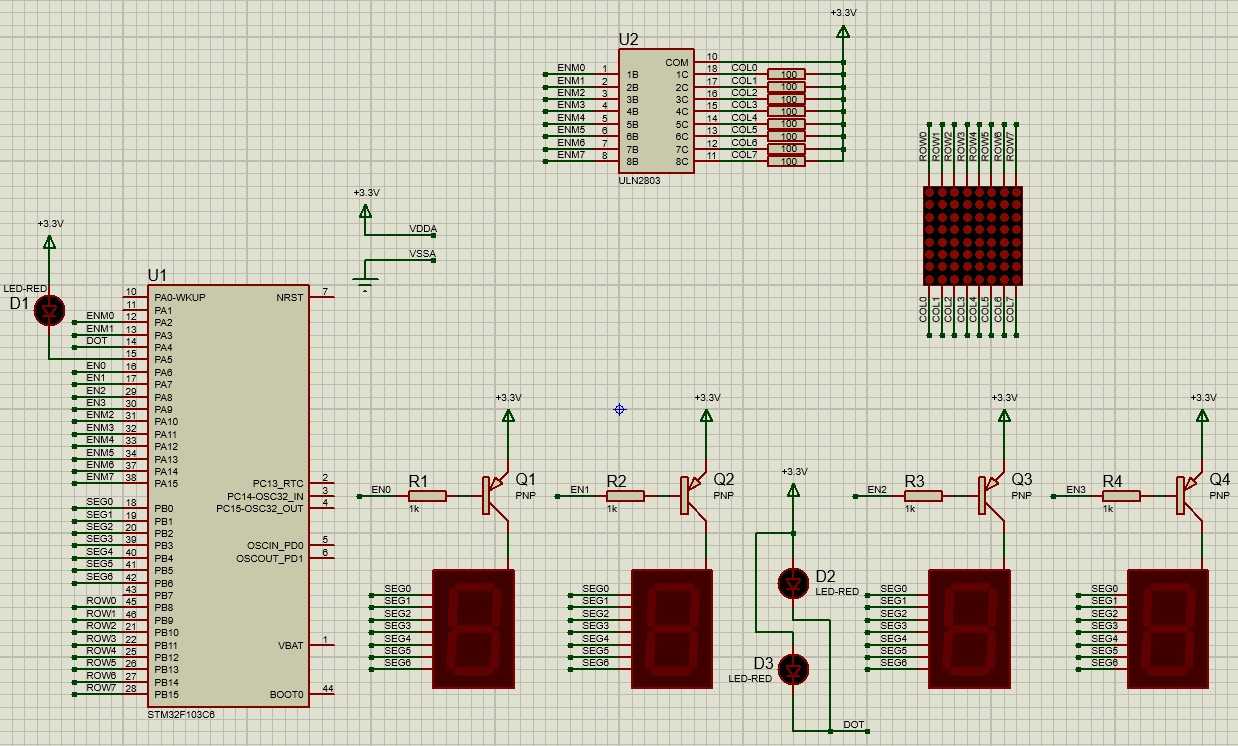
\includegraphics[width=0.8\linewidth]{pictures/schematic_ex09_10.jpg}
    \caption{{\textit{Proteus schematic with MATRIX-8X8-RED and ULN2803}}}
    \label{schematic_ex09}
\end{figure}

\textbf{Report 2: } Implement the function, updateLEDMatrix(int index), which is similarly  to 4 seven led segments.

\begin{lstlisting}[caption=Function to display data on LED Matrix]
const int MAX_LED_MATRIX = 8;
int index_led_matrix = 0;
uint8_t matrix_buffer[8] = {0x01, 0x02, 0x03, 0x04, 0x05, 0x06, 0x07, 0x08};
void updateLEDMatrix(int index){
    switch (index){
        case 0:
            break;
        case 1:
            break;
        case 2:
            break;
        case 3:
            break;
        case 4:
            break;
        case 5:
            break;
        case 6:
            break;
        case 7:
            break;
        default:
            break;
    }
}
\end{lstlisting}

Student are free to choose the invoking frequency of this function. However, this function is supposed to invoked in main function. Finally, please update the \textbf{matrix\_buffer} to display character \textbf{"A"}.\\

- Before the full implementation, we will go through a brief about the component \texttt{MATRIX-8X8-RED} (which is implemented in \textit{Figure 2.6}, not the example).

- After a few tests, we found out that \texttt{MATRIX-8X8-RED} interacted with \texttt{uint8\_t matrix\_buffer[8]} by converting hex value to binary base on the rows.

- For better illustration, we indicate the component by a 2x2 matrix, with "." states for 0 and "$\blacksquare$" states for 1.

\begin{table}[H]
\centering
\caption{Illustration of \texttt{MATRIX-8X8-RED}'s LEDs by a 2x2 matrix}
\begin{tabular}{c|cccccccc}
    & x0 & x1 & x2 & x3 & x4 & x5 & x6 & x7 \\ \hline
y0 & . & . & . & . & . & . & . & . \\
y1 & . & . & . & . & . & . & . & . \\
y2 & . & . & . & . & . & . & . & . \\
y3 & . & . & . & . & . & . & . & . \\
y4 & . & . & . & . & . & . & . & . \\
y5 & . & . & . & . & . & . & . & . \\
y6 & . & . & . & . & . & . & . & . \\
y7 & . & . & . & . & . & . & . & . \\
\end{tabular}
\end{table}

- Then we can display for the character A:

\begin{table}[H]
\centering
\caption{Sample of a character A on MATRIX-8X8-RED}
\begin{tabular}{c|cccccccc|cc}
    & x0 & x1 & x2 & x3 & x4 & x5 & x6 & x7 & Binary & HEX value\\ \hline
y0 & . & . & . & $\blacksquare$ & $\blacksquare$ & . & . & . & 00011000 & 0x18\\
y1 & . & . & $\blacksquare$ & $\blacksquare$ & $\blacksquare$ & $\blacksquare$ & . & . & 00111100 & 0x3C\\
y2 & . & $\blacksquare$ & $\blacksquare$ & . & . & $\blacksquare$ & $\blacksquare$ & . & 01100110 & 0x66\\
y3 & $\blacksquare$ & $\blacksquare$ & . & . & . & . & $\blacksquare$ & $\blacksquare$ & 11000011 & 0xC3\\
y4 & $\blacksquare$ & $\blacksquare$ & . & . & . & . & $\blacksquare$ & $\blacksquare$ & 11000011 & 0xC3\\
y5 & $\blacksquare$ & $\blacksquare$ & $\blacksquare$ & $\blacksquare$ & $\blacksquare$ & $\blacksquare$ & $\blacksquare$ & $\blacksquare$ & 11111111 & 0xFF\\
y6 & $\blacksquare$ & $\blacksquare$ & . & . & . & . & $\blacksquare$ & $\blacksquare$ & 11000011 & 0xC3\\
y7 & $\blacksquare$ & $\blacksquare$ & . & . & . & . & $\blacksquare$ & $\blacksquare$ & 11000011 & 0xC3\\
\end{tabular}
\end{table}

- For this exercise, we set the frequency $f = 12.5 $Hz for the MATRIX-8X8-RED. For details, please check out \texttt{latex/main\_code/ex09.txt}

\begin{lstlisting}[language=c,caption={Updates variables and functions for the software timer}]
//###################################################
// From exercise 3.6
int timer2_counter = 0, timer2_flag = 0;
void setTimer2(int duration) { timer2_counter = duration / TIMER_CYCLE; timer2_flag = 0; }

void timer_run()
{
	if(timer0_counter > 0) { timer0_counter--; if(timer0_counter == 0) timer0_flag = 1;	}
    if(timer1_counter > 0) { timer1_counter--; if(timer1_counter == 0) timer1_flag = 1; }
    if(timer2_counter > 0) { timer2_counter--; if(timer2_counter == 0) timer2_flag = 1; }
}
\end{lstlisting}

\vspace{1em}

\begin{lstlisting}[language=c,caption={Initialization for updateLEDMatrix(int index)}]
//###################################################
// From exercise 3.9

SegPin enm[8] =
{
    {ENM0_GPIO_Port, ENM0_Pin}, {ENM1_GPIO_Port, ENM1_Pin},
    {ENM2_GPIO_Port, ENM2_Pin}, {ENM3_GPIO_Port, ENM3_Pin},
    {ENM4_GPIO_Port, ENM4_Pin}, {ENM5_GPIO_Port, ENM5_Pin},
    {ENM6_GPIO_Port, ENM6_Pin}, {ENM7_GPIO_Port, ENM7_Pin},
};


SegPin row[8] =
{
    {ROW0_GPIO_Port, ROW0_Pin}, {ROW1_GPIO_Port, ROW1_Pin},
    {ROW2_GPIO_Port, ROW2_Pin}, {ROW3_GPIO_Port, ROW3_Pin},
    {ROW4_GPIO_Port, ROW4_Pin}, {ROW5_GPIO_Port, ROW5_Pin},
    {ROW6_GPIO_Port, ROW6_Pin}, {ROW7_GPIO_Port, ROW7_Pin},
};


void displayRow(uint8_t pattern)
{
    HAL_GPIO_WritePin(ENM0_GPIO_Port, ENM0_Pin, GPIO_PIN_RESET);
    HAL_GPIO_WritePin(ENM1_GPIO_Port, ENM1_Pin, GPIO_PIN_RESET);
    HAL_GPIO_WritePin(ENM2_GPIO_Port, ENM2_Pin, GPIO_PIN_RESET);
    HAL_GPIO_WritePin(ENM3_GPIO_Port, ENM3_Pin, GPIO_PIN_RESET);
    HAL_GPIO_WritePin(ENM4_GPIO_Port, ENM4_Pin, GPIO_PIN_RESET);
    HAL_GPIO_WritePin(ENM5_GPIO_Port, ENM5_Pin, GPIO_PIN_RESET);
    HAL_GPIO_WritePin(ENM6_GPIO_Port, ENM6_Pin, GPIO_PIN_RESET);
    HAL_GPIO_WritePin(ENM7_GPIO_Port, ENM7_Pin, GPIO_PIN_RESET);

    for (int r = 0; r < 8; r++)
        HAL_GPIO_WritePin(row[r].port, row[r].pin, ((pattern >> r) & 1) ? GPIO_PIN_SET : GPIO_PIN_RESET);
}


// ==================================================
\end{lstlisting}

\vspace{1em}

\begin{lstlisting}[language=c,caption={Implementation of \texttt{updateLEDMatrix()} for displaying 'A'}]
// The implementation also includes the adjustment of matrix\_buffer[8] to display the character 'A'.
const int MAX_LED_MATRIX = 8;
int index_led_matrix = 0;
uint8_t matrix_buffer[8] = {0x18, 0x3C, 0x66, 0xC3, 0xC3, 0xFF, 0xC3, 0xC3};
// Exercise example:		uint8_t matrix_buffer[8] = {0x01, 0x02, 0x03, 0x04, 0x05, 0x06, 0x07, 0x08};
// For display letter A:	uint8_t matrix_buffer[8] = {0x18, 0x3C, 0x66, 0xC3, 0xC3, 0xFF, 0xC3, 0xC3};

void updateLEDMatrix(int index)
{
	switch (index)
	{
		case 0:
			displayRow(matrix_buffer[0]);
			HAL_GPIO_WritePin(ENM0_GPIO_Port, ENM0_Pin, GPIO_PIN_SET);
			break;
		case 1:
			displayRow(matrix_buffer[1]);
			HAL_GPIO_WritePin(ENM1_GPIO_Port, ENM1_Pin, GPIO_PIN_SET);
			break;
		case 2:
			displayRow(matrix_buffer[2]);
			HAL_GPIO_WritePin(ENM2_GPIO_Port, ENM2_Pin, GPIO_PIN_SET);
			break;
		case 3:
			displayRow(matrix_buffer[3]);
			HAL_GPIO_WritePin(ENM3_GPIO_Port, ENM3_Pin, GPIO_PIN_SET);
			break;
		case 4:
			displayRow(matrix_buffer[4]);
			HAL_GPIO_WritePin(ENM4_GPIO_Port, ENM4_Pin, GPIO_PIN_SET);
			break;
		case 5:
			displayRow(matrix_buffer[5]);
			HAL_GPIO_WritePin(ENM5_GPIO_Port, ENM5_Pin, GPIO_PIN_SET);
			break;
		case 6:
			displayRow(matrix_buffer[6]);
			HAL_GPIO_WritePin(ENM6_GPIO_Port, ENM6_Pin, GPIO_PIN_SET);
			break;
		case 7:
			displayRow(matrix_buffer[7]);
			HAL_GPIO_WritePin(ENM7_GPIO_Port, ENM7_Pin, GPIO_PIN_SET);
			break;
		default:
			break;
	}
}
\end{lstlisting}

\vspace{1em}

- Finally, with all of that, we just need to call in \texttt{int main(void)}.

\begin{lstlisting}[language=c,caption={Implementation for while loop}]
/* USER CODE BEGIN 2 */
HAL_TIM_Base_Start_IT(&htim2);
setTimer0(1000);
setTimer1(250); // add from 3.8
setTimer2(10);	// add from 3.9


while (1)
{
	if (timer0_flag == 1)
	{
		setTimer0(1000);

		second++;
		if (second >= 60) { second = 0; minute++; }
		if (minute >= 60) { minute = 0; hour++; }
		if (hour >= 24)   { hour = 0; }

		HAL_GPIO_TogglePin(DOT_GPIO_Port, DOT_Pin);
	}
	updateClockBuffer();


    if (timer1_flag == 1)
    {
        setTimer1(250);

        update7SEG(index_led++);
        HAL_GPIO_TogglePin(LED_GPIO_Port, LED_Pin);
        if (index_led >= MAX_LED) index_led = 0;
    }


    if (timer2_flag == 1)
    {
        setTimer2(10);
        updateLEDMatrix(index_led_matrix++);
        if (index_led_matrix >= MAX_LED_MATRIX) index_led_matrix = 0;
    }
}
\end{lstlisting}










\subsection{Exercise 10}
Create an animation on LED matrix, for example, the character is shifted to the left. 

\textbf{Report 1: } Briefly describe your solution and present your source code in the report.\\

- For this exercise, we came to a solution is to make the character shift to the left.

- In order to this, we can use a way is to shift bits, since the matrix LEDs work as binaries. We will take off the left-most column -> shift the whole matrix to the left -> put the take-out to the right-most.

\begin{lstlisting}[language=c,caption={Implementation for the shift bits function}]
void shiftLeft(void)
{
    for (int i = 0; i < MAX_LED_MATRIX; i++)
    {
        uint8_t b = matrix_buffer[i];
        matrix_buffer[i] = (b >> 1) | (b << 7);
    }
}
\end{lstlisting}

- In the loop:
\begin{itemize}
    \item \texttt{b >> 1} does the “move left” part.
    \item \texttt{b << 7} rescues the cell that would have been lost and puts it on the far right.
    \item \texttt{|} merges the two results into one row.
\end{itemize}
so the whole \texttt{matrix\_buffer[i] = (b >> 1) | (b << 7);} is just updating the value from the combanation of two different results to make like it is shifting at row \texttt{i}.

- Then we just need to make a new software timer.\newline
(\textit{or you can just synchronize this one with the scanning 7-segment LEDs one if you are lazy})

\begin{lstlisting}[language=c,caption={Updates variables and functions for the software timer}]
//###################################################
// From exercise 3.6
int timer3_counter = 0, timer3_flag = 0;
void setTimer3(int duration) { timer3_counter = duration / TIMER_CYCLE; timer3_flag = 0; }

void timer_run()
{
	if(timer0_counter > 0) { timer0_counter--; if(timer0_counter == 0) timer0_flag = 1;	}
    if(timer1_counter > 0) { timer1_counter--; if(timer1_counter == 0) timer1_flag = 1; }
    if(timer2_counter > 0) { timer2_counter--; if(timer2_counter == 0) timer2_flag = 1; }
    if(timer3_counter > 0) { timer3_counter--; if(timer3_counter == 0) timer3_flag = 1; }
}
\end{lstlisting}

\vspace{1em}

\begin{lstlisting}[language=c,caption={Implementation for while loop}]
/* USER CODE BEGIN 2 */
HAL_TIM_Base_Start_IT(&htim2);
setTimer0(1000);
setTimer1(250); // add from 3.8
setTimer2(10);	// add from 3.9
setTimer2(200);	// add from 3.10

while (1)
{
    /*Old 3.9 code*/


    if (timer3_flag == 1)
    {
        setTimer3(200);
        shiftLeft();
    }
}
\end{lstlisting}












